\section{Vstavané systémy a mikrokontroléry}
\noindent
Pojmom vstavaný systém označujeme spojenie počítačového hardvéru a softvéru, ktorý je navrhnutý tak, aby vykonával vyhradenú aktivitu. Tá môže byť súčasťou komplexného systému, avšak môže fungovať aj samostatne. Jadrom vstaveného systému
je integrovaný obvod určený na vykonávanie výpočtov pre operácie v reálnom čase \cite{WhatEmbeddedSystem}. \par
Mikrokontrolér je procesor, ktorý je vybavený pamäťou, časovačmi, radičom prerušení, I/O pinmi a rôznymi ďalšími periférnymi
zariadeniami. Vďaka tomu dokáže fungovať samostatne a vykonávať rôzne úlohy. Mikrokontroléry tiež obsahujú bitové operácie, ktoré nám umožňujú zmeniť jeden bit v rámci bajtu bez toho, aby sme sa dotkli ostatných bitov. \par
Všetky prvky mikrokontroléra sú integrované na jednom čipe, čím sa šetrí miesto.
To vedie k nižším nákladom a kratšej dobe vývoja. Tým sa šetrí čas a aj peniaze čo je hlavný
dôvod existencie a popularity rôznych mikrokontrolérov. Medzi ďalšie výhody patrí nižšia spotreba energie,
jednoduchosť modernizácie komponentov mikrokontroléra a vyššia spoľahlivosť
celého systému. Tieto výhody patria medzi dôležité aspekty vstavaných systémov. \par
K nevýhodám môžeme zaradiť rýchlosť zariadenia, keďže tá bude takmer vždy
nižšia ako by sme vedeli dosiahnuť len pomocou hardvérového riešenia. Väčšina aplikácii, a najmä tie, ktoré vyžadujú istý druh ľudskej interakcie, nepotrebujú
dosiahnuť také rýchle reakčné časy. Preto je mikrokontrolér pre ne dobrou voľbou
\cite{guntherIntroductionMicrocontrollers2007}.

\subsection{Typy mikrokontrolérov}
\noindent
V dnešnej dobe poznáme niekoľko typov mikrokontrolérov. Medzi najznámejšie patria:
\begin{itemize}
    \item PIC mikrokontrolér
    \item ARM mikrokontrolér
    \item AVR mikrokontrolér
\end{itemize}

\subsubsection{PIC mikrokontrolér}
\noindent
PIC je rodina mikrokontrolérov vyrábaných technológiou mikročipov, pôvodne navrhnutou pre vývoj všobecných elektronických zariadení.
Názov PIC pôvodne označoval Peripheral Interface Controller a v súčasnosti je
rozšírený ako Programmable Intelligent Computer. Zariadenie PIC je známe pre
svoju nízku cenu, širokú dostupnosť a veľkú používateľskú základňu. \par

Z periférnych zariadení je tento mikrokontrolér vybavený:
\begin{itemize}
    \item Tromi časovačmi
    \item Dvomi tzv. Capture/Compare/PWM modulmi
    \item 10 bitovým analógovo-digitálnym prevodníkom
    \item Synchrónnym sériovým portom s podporou I2C master/slave komunikácie
    \item 8 bitovým paralelným slave portom
\end{itemize}

Medzi výhody PIC patrí spoľahlivosť. Zároveň je aj veľmi rýchly vďaka použitiu architektúry RISC.
Spotreba energie je taktiež menšia ak ju porovnáme so spotrebou iných mikrokontrolérov. K nevýhodám môžeme zaradiť dĺžku programu.
Tá bude väčšia práve kvôli použitiu RISC architektúry (35 inštrukcií) \cite{shidlingDifferentTypesMicrocontrollers2020}.

\subsubsection{ARM mikrokontrolér}
\noindent
Názov ARM označuje Advanced Risk machine. ARM mikrokontrolér taktiež využíva architektúru procesora RISC. Procesor ARM patrí medzi jeden z najrozsiahlejších
a najviac licencovaných procesorov na svete. Prvýkrát bol vyvinutý v roku 1978 Cambridgskou univerzitou. Firma ARM v súčasnosti vyvíja ARM architektúru a
licencuje ju rôznym ďalším spoločnostiam, ktoré vyvíjajú svoje vlastné produkty.
Procesory ARM majú menší počet tranzistorov kvôli menšiemu počtu podporovaných inštrukcií. Vďaka tomu je ARM procesor menší ako rôzne iné modely, a preto sa nachádza v obrovskom množstve elektronických zariadení. Spojením procesora ARM
s RAM a ROM pamäťou a ďalšími periférnymi zariadeniami dostaneme ARM mikrokontrolér.\par

V porovnaní s inými procesormi sú lacné a zároveň majú menšiu energetickú spotrebu. Z toho vyplýva aj väčšia výdrž batérie.
Medzi nevýhody určite patrí to, že architektúra ARM nie je kompatibilná s architektúrou x86 \cite{shidlingDifferentTypesMicrocontrollers2020}.

\subsubsection{AVR mikrokontrolér}
\noindent
AVR bol vyvinutý v roku 1996 spoločnosťou Atmel Corporation. Názov AVR je odvodený od mien vývojarov, ktorí na ňom pracovali.
Je to skratka od  Alf-Egil Bogen Vegan Wollan RISC mikrokontrolér.
Taktiež je známy aj pod názvom Advanced Virtual RISC. AVR mikrokontrolér je dostupný v troch kategóriách:
\begin{itemize}
    \item TinyAVR: Najmenší dostupný model. Je určený len pre jednoduché aplikácie.
    \item MegaAVR: Najpopulárnejší model AVR mikrokontrolérov. Má väčšie množstvo pamäte a viac zabudovaných periférnych zariadení. Je vhodný pre stredné náročné až zložité aplikácie.
    \item XmegaAVR: Je určený na komerčné použitie pre komplexné aplikácie, ktoré vyžadujú veľké množstvo pamäte a vysokú rýchlosť procesora.
\end{itemize}

AVR je jednou z prvých architekúr mikrokontrolérov, ktoré používajú zabudovanú flash pamäť, narozdiel od jednorazovo programovateľnej pamäte ROM, EPROM alebo EEPROM, ktoré v tom čase používali ostatné mikrokontroléry.
\par
Medzi hlavné výhody patrí cena, jednoduchosť používania a v neposlednom rade aj možnosť výberu rôznych typov na základe užívateľských požiadaviek \cite{shidlingDifferentTypesMicrocontrollers2020}. AVR je taktiež využívané platformou Arduino \cite{AVRVsArduinoWhich2017}.


\section{Prerušenia}
\noindent Vo vstavaných systémoch prerušenie upozorní procesor na udalosť, ktorá nastala a je potrebné, aby jej procesor venoval pozornosť. Často ide o signály vygenerované perifériami procesora. Procesor na prerušenie zareaguje pozastavením vykonávania aktuálnej aktivity, uložením jej stavu a začatím vykonávania kódu na inej pamäťovej adrese \cite{wangAutomaticDetectionValidation2017}. \par 
Táto adresa je definovaná v takzvanom \textit{vektore prerušení} (interrupt vector). \textit{Vektor prerušení} je konfiguravateľné alebo pevne dané miesto v pamäti, ktoré špecifikuje adresu, kde má procesor pokračovať vo vykonávaní kódu. Každé podporované prerušenie sa musí nachádzať v tomto vektore. Blok pamäte kam odkazuje vektor prerušení, sa nazýva \textit{obsluha prerušenia}. V anglickej literatúre sa používa výraz \textit{interrupt service routine} \textit{(ISR)}, preto aj my budeme ďalej používať skratku  ISR. Po vykonaní  ISR sa procesor vráti k predtým vykonávanej aktivite. \par
\textit{Radič prerušení} je periférne zariadenie, ktoré spravuje prerušenia pre procesor. Niektoré architektúry procesorov majú integrovaný sofistikovaný radič prerušení (napríklad AVR alebo MSP430), zatiaľ čo iné obsahujú iba základný ovládač, ktorý si vyžaduje ďalší externý radič prerušení (napríklad ARM alebo x86). \par
Prerušenie je v stave \textit{čakania}, ak daná udalosť nastala a radič prerušení dané prerušenie zaregistroval, avšak ešte sa nezačalo vykonávanie ISR.  O \textit{zmeškanom prerušení} hovoríme, keď udalosť prerušenia nastala, ale radič prerušení sa o tom nedozvedel. Toto väčšinov nastáva v situácii, keď je prerušenie v stave čakania a udalosť nastane znova. \par
Prerušenie je \textit{zakázané}, keď je na hardvérovej úrovni zabránené spusteniu prerušenia. Vo všeobecnosti, väčšina prerušení má svoj dedikovaný bit v hardvérových registroch, ktorý povoľuje, respektíve zakazuje vykonanie prerušenia. Na väčšine procesorov je taktiež možné vypnúť všetky prerušenia vynulovaním bitu, ktorý globálne zakazuje/povoľuje prerušenia. Tento bit sa nazýva aj \textit{master interrupt enable bit}.\par 
Prerušenie nastane pri splnení nasledujúcich podmienok:
\begin{enumerate}
    \item Master interrupt enable bit je nastavený.
    \item Dedikovaný bit prerušenia je nastavený.
    \item Prerušenie je v stave čakania.
    \item Procesor sa nachádza v stave medzi vykonaním dvoch inštrukcií alebo vykonáva inštrukciu, ktorú je možné prerušiť.
    \item Nenastalo žiadne prerušenie, ktoré splnilo podmienky 1-4 a má vyššiu prioritu.
\end{enumerate} \par

\textit{Latencia} prerušenia je časový interval od momentu kedy boli splnené podmienky vykonania prerušenia až po chvíľu začatia vykonávania ISR daného prerušenia. Ak sa objaví ďalšie prerušenie s vyššou prioritou, latencia prerušenia s nižšou prioritou môže byť veľká. K dĺžke latencie prispievajú aj vyššie spomínané podmienky vykonania prerušenia, keďže kontrola či sú bity nastavené alebo dokončenie vykonávania aktuálnej inštrukcie procesorom trvá nejaký čas. \par
Veľká väčšina procesorov podporuje aj prerušenia, ktoré nie je môžné vypnúť (non-maskable interrupt - NMI). Používajú sa v prípade nastania fatálnych chýb z, ktorých nie je možné žiadnym spôsobom vykonať nápravu programu
\cite{regehrSafeStructuredUse2007}. \par
Prerušenia je možné vnímať aj ako udalosti. Pri ich využívaní v programe je preto možné hovoriť o programovaní pomocou udalosťami riadenej paradigmy. Takýto program je možné označiť ako \begin{math}P=Task || ISR\end{math}, kde \begin{math}Task\end{math} je hlavný program pozostávajúci z jednej alebo viacerých úloh (vlákien) a  \begin{math}ISR\end{math} kde \begin{math}ISR=ISR_1||ISR_2||ISR_3||..||ISR_N\end{math} sú obsluhy prerušení.
Indexy daných \begin{math}ISR\end{math} predstavujú číslo prerušenia. Čím je číslo väčšie, tým menšiu prioritu dané prerušenie má \cite{wangAutomaticDetectionValidation2017}. \par Prerušenia sú väčšinovo využívané na indikovanie dvoch typov udalostí. Prvou je udalosť vykonaná používateľom, kde patrí napríklad stlačenie tlačidla. Druhou je prijatie dát z periferného zariadenia. Ako príklad môžeme uviesť UART protokol \cite{wangAutomaticDetectionValidation2017}.
\setcounter{tocdepth}{4}
\setcounter{secnumdepth}{4}

\subsection{AVR časovače a počítadlá}
\noindent

Ako názov napovedá, časovače sú určené na meranie času. Často ich nazývame aj počítadlá,
pretože vo svojom základnom princípe časovače len počítajú počet dokončených periód zdrojových hodín.
Každý časovač má svoj vlastný register, kde je uložená jeho aktuálna hodnota a taktiež každý potrebuje zdroj hodín. V mikrokontroléroch často existuje niekoľko možných zdrojov
hodín a ich výber je možné určiť pomocou prepínača. Niektoré mikrokontroléry umožňujú aj použitie
externých hodín \cite{IntroductionMicrocontrollerTimers}. Pri rôznych architektúrach sa môže spôsob fungovania časovačov líšiť. V tejto diplomovej práci sa budeme venovať
mikrokontroléru s architektúrou AVR, preto aj nasledujúci opis fungovania časovačov sa vzťahuje na architektúru AVR.\par
Fungovanie časovača si najlepšie opíšeme na konkrétnom príklade.
Uvažujme časovač s 16-bitovým registrom a zdrojom hodín s frekvenciou 1 kHz. Po každom uplynutí cyklu v hodinách, časovač
zvýši hodnotu uloženú v registri o 1. Dĺžku jedného cyklu časovača je možné vyjadriť vzorcom:

\begin{equation}
    \begin{aligned}
        Dĺžka\:cyklu = \frac{1}{Frekvencia\:hodín}
    \end{aligned}
\end{equation}

To znamená, že najkratší časový úsek, ktorý je možné pomocou časovača odmerať sa
rovná dĺžke periódy vstupných hodín. V našom príklade s hodinami s frekvenciou 1 kilohertz je dĺžka periódy nasledovná:
\begin{equation}
    \begin{aligned}
        Dĺžka\:cyklu & = \frac{1}{Frekvencia\:hodín} \\
                     & = \frac{1}{1kHz}              \\
                     & = \frac{1}{ 1000 Hz}          \\
                     & =  0.001\:sekundy
    \end{aligned}
\end{equation}
Dĺžka periódy je 0.001 sekundy. Z toho vyplýva, že časovač je schopný odmerať dĺžku času, ktorý je násobkom 0.001. Ak necháme časovač napočítať do 100, potrvá to 100 krát 0.001 sekundy, čiže 0.1 sekundy \cite{cameraNewbieGuideAVR2015}.
Tu treba poznamenať, že v našom príklade počítame s frekvenciou 1kHz, čo je pomerne nízka frekvencia a dnešné mikrokontroléry sú podstatne rýchlejšie.
Ako príklad uvedieme mikrokontrolér Arduino Mega2560, ktorý používa frekvenciu 16MHz čo je rádovo viac ako 1kHz \cite{ArduinoMega2560}.
\par Pre reálnejšiu predstavu preto pokračujme v našom príklade s časovačom s frekvenciou 1MHz. Časovač má k dispozícii 16-bitový register. Maximálny počet
možných hodnôt v registri je teda $2^{16}$ (65536, maximálna hodnota je 65365).
Po dosiahnutí maximálnej hodnoty register pretečie a časovač začne počítať znova od 0.
\begin{figure}[!h]
    \centering
    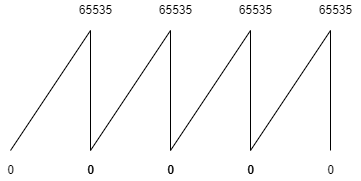
\includegraphics[width=0.70\textwidth]{img/timer.png}
    \caption{Zmena hodnoty v 16 bitovom registri časovača}
    \label{figure:timer1}
\end{figure}

Pri hodinách s frekvenciou 1MHz časovač dosiahne maximálnu hodnotu registra približne každých 66 milisekúnd a dĺžka jedného cyklu je $\frac{1}{1000000}$ sekundy, čo je 1 mikrosekunda \cite{cameraNewbieGuideAVR2015}.

\subsubsection{Preddelička}
\noindent \par
Pri použití 16-bitového registra je 66 milisekúnd najdlhší časový interval, ktorý dokážeme odmerať pokým register nepretečie a časovač nezačne počítať od 0.
Pre nás ľudí je to veľmi krátky časový úsek. Často chceme dosiahnuť interval, ktorý je dlhší a pre nás badateľný. Príkladom takého intervalu je 1 sekunda.
Existuje viacero spôsobov ako tento interval dosiahnuť. Jedným z nich je použitie preddeličky (v anglickej literatúre sa používa termín prescaler).
\par
Preddelička je súčasťou obvodu časovača, ktorý nám umožňuje preskočiť periódy zdrojových hodín o mocninu 2, čím sa zníži frekvencia,
ale zároveň dostaneme dlhší rozsah časovača.
Hodnoty preddeličky bývajú pevne dané a často sú to hodnoty 1, 8, 64, 256 a 1024. Vzorec pre výpočet dĺžky cyklu spolu s preddeličkou je nasledovný \cite{atmelATmega64012801281}:

\begin{equation} \label{eq:cycle-length}
    \begin{aligned}
        Dĺžka\:cyklu & = \frac{1}{\frac{Frekvencia\:hodín}{Preddelička}} \\
                     & = \frac{Preddelička}{Frekvencia\:hodín}           \\
    \end{aligned}
\end{equation}

Pre časovač s frekvenciou 1MHz a hodnotami preddeličky 1, 8, 64, 256 s 1024 môžeme zostrojiť nasledujúcu tabuľku:
\begin{table}[!htbp]
    \begin{center}
        \begin{tabular}{|c|c|}
            \hline
            Hodnota preddeličky & Dĺžka cyklu časovača \\
            \hline
            1                   & 1 $\mu s$            \\
            8                   & 8 $\mu s$            \\
            64                  & 64 $\mu s$           \\
            256                 & 256 $\mu s$          \\
            1024                & 1024 $\mu s$         \\
            \hline
        \end{tabular}
        \caption{Dĺžka cyklu 1MHz časovača pri rôznych hodnotách preddeličky}
        \label{table:timerPrescaler}
    \end{center}
\end{table}

Pre dosiahnutie 1 sekundového intervalu potrebujeme poznať aj hodnotu registra,
pri ktorej tento interval uplynie. Tú dostaneme použitím nasledujúceho vzorca:

\begin{equation} \label{eq:register-value}
    \begin{aligned}
        Hodnota\:registra & = \frac{ \frac{1}{Cieľová\:frekvencia}} { \frac{Preddelička}{Frekvencia\:hodín}} - 1 \\
                          & = (\frac{Frekvencia\:hodín}{Preddelička \times Cieľová\:frekvencia}) - 1             \\
    \end{aligned}
\end{equation}

Časovače AVR aktualizujú svoju hodnotu iba pri každom tiknutí vstupných hodín.
Je teda potrebný tik, aby sa hodnota časovača dostala z maximálnej hodnoty späť na nulu. Preto v znázornenom vzorci
musíme znížiť počet tikov o jeden \cite{atmelATmega64012801281}. \par

Teraz sa vráťme späť k tomu, ako dosiahneme interval 1 sekundy.
Potrebujeme zistiť či existuje hodnota preddeličky, ktorá poskytne presné oneskorenie 1 Hz. Jeden Hertz je rovný jednému cyklu za sekundu. Na výpočet použijeme vzorec
č.\ref{eq:register-value} a výsledky týchto výpočtov sú uvedené v tabuľku č. \ref{table:timerPrescalerValues}:

\begin{table}[!htbp]
    \begin{center}
        \begin{tabular}{|c|c|}
            \hline
            Hodnota preddeličky & Hodnota registra časovača \\
            \hline
            1                   & 999999                    \\
            8                   & 124999                    \\
            64                  & 15624                     \\
            256                 & 3905,25                   \\
            1024                & 975,5625                  \\
            \hline
        \end{tabular}
        \caption{Potrebná hodnota v registri 1MHz časovača pre dosiahnutie 1 sekundového intervalu}
        \label{table:timerPrescalerValues}
    \end{center}
\end{table}

Pri pohľade na tabuľku môžeme hneď usúdiť, že preddeličky s hodnotou 256 a 1024 nie sú vhodné pre dosiahnutie nášho cieľa. Hodnota v registri je vždy celé kladné číslo, a preto nemôžme tieto hodnoty použiť. Ďalším kritériom pre výber preddeličky je veľkosť
vypočítanej hodnoty. Náš časovač používa 16-bitový register, ktorého maximálna hodnota je $2^{16} -1$ (65365).
Ostáva nám teda len jedna možnosť preddeličky, a to 64. Preddeličky s hodnotou 1 a 8 vyžadujú hodnotu registra väčšiu ako je schopný uložiť.
Teda, pre dosiahnutie jedno sekundového intervalu pomocou 16 bitového časovača s frekvenciou 1MHz potrebujeme použiť preddeličku s hodnotou 64.
1 sekundu časovač dosiahne po napočítaní do 15624. \par
Čo však v prípade ak chceme dosiahnuť dlho trvajúce intervaly? Hodinu, deň, týždeň, mesiac prípadne rok?
V tomto prípade je možné implementovať preddeličku aj softvérovo. Pre jednoduchšie vysvetlenie si riešenie problému ukážeme na príklade. Uvažujme rovnaké parametre časovača: 1MHz frekvencia, 16 bitový register. Chceme dosiahnuť časový interval jednej hodiny. Pomocou vyššie popísanej techniky vytvoríme interval 1 sekundy.
Po každom uplynutí intervalu zvýšime hodnotu nášho počítadlá. 1 hodina je 3600 sekúnd. Teda vieme, že pokiaľ naše počítadlo dosiahne hodnotu 3600 ubehla 1 hodina.
Pseudokód danej implementácie by mohol vyzerať nasledovne:
\begin{lstlisting}[
    language=c
  ]  
Initialise counter to 0
WHILE forever
    IF timer value IS EQUAL TO 1 sec THEN
        Increment counter
        Reset timer
        IF counter value IS EQUAL TO 3600 THEN
            // 1 HOUR HAS PASSED
            Reset counter
        END IF
    END IF
END WHILE
\end{lstlisting}
Pri takejto implementácii je potrebné dať si pozor aj na najmenšie odchýlky od základného intervalu, ktorý je nastavený pomocou hardvérovej preddeličky.
Aj najmenšia odchýlka môže po sčítaní znamenať veľkú nepresnosť v požadovanom konečnom intervale \cite{cameraNewbieGuideAVR2015}.

\subsubsection{Časovače a prerušenia} \label{subsec:timers-interrupts}
\noindent \par
Pomocou AVR časovačov existujú dva spôsoby ako vykonať kód v presne danom čase. Prvým je použitie cyklu.
Pri tejto metóde dochádza k neustálej kontrole hodnoty registra časovača. Ak register dosiahne požadovanú hodnotu, vieme, že požadovaný interval skončil
a je možné vykonať inú akciu/akcie. Druhou možnosťou je presunúť zodpovednosť toho, kedy je akciu potrebné vykonať na hardvér AVR mikrokontroléra.
To je možné dosiahnuť pomocou prerušení časovača. AVR časovače podporujú niekoľko druhov prerušení.
Najčastejšie ide o Overflow (pretečenie) a Compare and Capture (porovnanie a zachytenie) prerušenia \cite{atmelATmega64012801281}. \par
Overflow prerušenie nastáva pri pretečení registra časovača. Časovač napočíta do svojej maximálnej hodnoty a v nasledujúcom cykle sa hodnota registra nastaví na 0.
Pri tomto pretečení časovač nastaví bit vo svojom stavovom registri a na základe toho je informovaná hlavná aplikácia o udalosti, ktorá nastala. Ak je dané prerušenie
povolené a zároveň sú globálne povolené všetky prerušenia, tak mikrokontrolér prestane vykonávať aktuálnu činnosť a spustí obsluhu prerušenia. Takýmto spôsobom
ponecháme rozhodnutie o vypršaní časového intervalu na hardvér AVR. Ak nechceme používať prerušenia, možnosťou je aj neustála softvérová kontrola bitu časovača v kontrolnom registri.
Práve na základe tohto bitu hardvér AVR vyvolá obsluhu prerušenia \cite{atmelATmega64012801281}. Nevýhodou je, že zatiaľ čo v tejto metóde je procesor neustále zamestnaný kontrolou
hodnoty registra, v prípade prerušenia môže namiesto toho vykonávať inú prospešnú činnosť. \par
Pre zostavenie rovnice na výpočet časového intervalu pretečenia môžeme použiť vzorec č.\ref{eq:cycle-length}. Ten hovorí o dĺžke jedného cyklu. Ak teda dĺžku cyklu
vynásobíme počtom možných hodnôt, dostaneme časový interval potrebný na pretečenie registra:

\begin{equation} \label{eq:overflow-frequency}
    \begin{aligned}
        Časový\:interval\:pretečenia =  2^{Veľkosť\:registra}  \times \frac{Preddelička}{Frekvencia\:hodín}
    \end{aligned}
\end{equation}

V nasledujúcej tabuľke č.\ref{table:overflow-frequency} vidíme porovnanie frekvencií a časových intervalov pretečenia registra časovača. Pre zostrojenie tabuľky sme uvažovali 16 bitový časovač
s frekvenciou 1MHz.  Vidíme, že čím väčšia hodnota preddeličky, tým menšia frekvencia
pretečenia registra. Z takmer nebadateľnej hodnoty pre ľudí, milisekunda, sme sa dostali až k intervalu viac ako 1 minúty.

\begin{table}[!htbp]
    \begin{center}
        \begin{tabular}{|c|c|c|}
            \hline
            Hodnota preddeličky & Frekvencia & Časový interval \\
            \hline
            1                   & 15,259 Hz  & 65,5 ms         \\
            8                   & 1,907 Hz   & 0,524 s         \\
            64                  & 0,2384 Hz  & 4,195 s         \\
            256                 & 0,0596 Hz  & 16,78 s         \\
            1024                & 0,0149 Hz  & 67,11 s         \\
            \hline
        \end{tabular}
        \caption{Frekvencie pretečenia registra pri rôznom nastavení preddeličky}
        \label{table:overflow-frequency}
    \end{center}
\end{table}

Použitie overflow prerušenia si ukážeme na už spomínanom príklade dosiahnutia 1 sekundového intervalu. V predchádzajúcich kapitolách sme si ukázali,
že pri použití 16-bitového časovača s frekvenciou 1MHz je možné dosiahnuť 1 sekundový interval po napočítaní do 15625 spolu s použitím preddeličky s hodnotou 64.
Zároveň vieme, že maximálna hodnota registra je 65535 a pri následnom pretečení nastane prerušenie. Vieme teda, že ak časovač dosiahne maximálnu hodnotu registra každú
sekundu, aj prerušenie bude vykonané pravidelne v tomto intervale. Z toho vyplýva, že časovač nesmie začať počítať od 0 ale od inej, presne danej hodnoty.
Pre matematické vyjadrenie počiatočnej hodnoty registra použijeme vzorec č.\ref{eq:register-value}. Pri vzorci sme uvažovali počiatočnú hodnotu 0. Tentokrát chceme
dosiahnuť to, aby po uplynutí intervalu časovač dosiahol svoju maximálnu hodnotu. Vzorec pre tento výpočet bude teda nasledovný:

\begin{equation} \label{eq:start-value}
    \begin{aligned}
        Počiatočná\:hodnota =  (2^{Veľkosť\:registra} - 1) - (\frac{Frekvencia\:hodín}{Preddelička \times Cieľová\:frekvencia})
    \end{aligned}
\end{equation}

Čo v našom konkrétnom prípade predstavuje:

\begin{equation}
    \begin{aligned}
        Počiatočná\:hodnota & =  (2^{Veľkosť\:registra} - 1) - 15625 \\
                            & =  (2^{16} - 1) - 15625                \\
                            & =  65535 - 15625                       \\
                            & =  49910
    \end{aligned}
\end{equation}

Hodnotu 49910 zapíšeme do kontrolného registra časovača na začiatku programu a následne pri
každej obsluhe overflow prerušenia. Pseudokód 1 sekundového intervalu s použitím overflow prerušenia vyzerá nasledovne:

\begin{lstlisting}[
    label={lst:oveflow-interrupt},
    language=c]  
Enable timer overflow interrupt
Enable global interrupts
Set timer prescaler to 64
Set timer register value to 49910

WHILE forever
END WHILE

ISR Timer Overflow
    Set timer register value to 49910
    // Do some work
END ISR

\end{lstlisting}

Spomínané Compare and Capture prerušenie sa vzťahuje hlavne k CTC módu časovača, preto si ho predstavíme až v kapitole č.\ref{subsec:ctc-mode}.

\subsubsection{CTC mód} \label{subsec:ctc-mode}
\noindent \par
Doteraz opisovaný spôsob fungovania AVR časovača sa vzťahuje na tzv. normálny  mód. V tomto móde časovač ráta od 0 po maximálnu hodnotu.
Je to základný a najjednoduchší spôsob fungovania AVR časovačov. Preto sme si na ňom predstavili spôsob akým tieto časovače fungujú a akým spôsobom sa dajú prakticky
používať. Komplikovanejším módom je tzv. „Clear timer on Compare“ (vynulovanie časovača pri porovnaní) mód, označovaný ako CTC mód. \par
CTC mód na hardvérovej úrovni porovnáva aktuálnu hodnotu časovača s požadovanou hodnotou. Ide o hardvérové porovnanie, ktoré je značne rýchlejšie ako porovnanie
softvérové. Ak časovač požadovanú hodnotu dosiahne, CTC mód nastaví bit v stavovom registri
a zároveň vynuluje hodnotu časovača. Týmto nám významným spôsobom uľahčuje prácu s časovačom. Nemusíme sa totiž starať o vynulovanie hodnoty časovača ako sme si ukázali
v kapitole č.\ref{subsec:timers-interrupts}. Zároveň nám ostáva možnosť použitia prerušenia na vykonanie akcie. Ak povolíme CTC prerušenia, tak po zapísaní bitu
do stavového registra AVR vykoná obsluhu prerušenia Compare and Capture. Aktuálna hodnota časovača je porovnávaná s hodnotou alebo hodnotami v tzv. Output Compare registrami.
16 bitové časovače majú tieto registre tri. Označované sú ako Output Compare Register A, Output Compare Register B a Output Compare Register C. My ich ďalej budeme nazývať
porovnávací register A, B, C. V 8 bitových časovačoch nájdeme len prvé dva. Vďaka viacerým porovnávacím registrom, dokážeme jeden časovač využiť na generovanie viacerých
časových intervalov \cite{atmelATmega64012801281}. \par
Po každom tiku časovača je aktuálna hodnota  porovnaná s hodnotami v porovnávacích registroch. Každý porovnávací register funguje
samostatne a podporuje nezávislé generovanie prerušení. Je dôležité poznamenať, že hodnota časovača je vynulovaná len v prípade zhody hodnoty s porovnávacím registrom A.
To je obzvlášť dôležité ak chceme používať jeden časovač na generovanie viacerých intervalov. Ak by sme do porovnávacieho registra B zapísali hodnotu väčšiu ako
do porovnávacieho registra A, časovač nikdy nedosiahne hodnotu v registri B. Rovnako to platí aj pre register C. Z uvedeného taktiež vyplýva, že maximálna hodnota
časovača už nie je kapacita jeho registra, ale hodnota, ktorá je zapísaná v porovnávacom registri A \cite{atmelATmega64012801281}. \par
Ako príklad znovu využijeme 1 sekundový interval, označíme ho ako interval 1.
Pridáme k nemu ešte interval 200 milisekúnd, ktorý chceme, aby odštartoval v rovnaký moment ako 1 sekundového interval. Pomenujeme ho ako interval 2. Pre jednoduchšiu
predstavu je na obrázku č.\ref{figure:interval-timeline} zobrazená časová os spolu s označenými intervalmi.


\begin{figure}[!h]
    \centering
    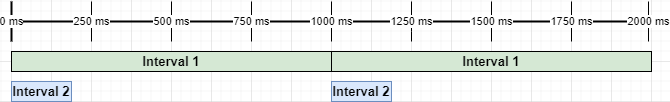
\includegraphics[width=0.85\textwidth]{img/interval-timeline.drawio.png}
    \caption{Časová os požadovaných intervalov}
    \label{figure:interval-timeline}
\end{figure}

Jeden časovač chceme použiť na dva rôzne intervaly. Preto v CTC móde potrebujeme 2 porovnávacie registre. Použijeme register A a porovnávací register B. Znovu uvažujeme
16 bitový časovač s frekvenciou 1MHz. V predchádzajúcich kapitolách sme vypočítali, že pri použití preddeličky s hodnotou 64, časovač dosiahne 1 sekundový interval
po napočítaní do 15624. Potrebujeme ešte vypočítať porovnávaciu hodnotu pre interval 200 milisekúnd. Použijeme na to vzorec č.\ref{eq:register-value}.

\begin{equation}
    \begin{aligned}
        Hodnota\:registra & = (\frac{Frekvencia\:hodín}{Preddelička \times Cieľová\:frekvencia}) - 1 \\
                          & = (\frac{1 \times 10^{6}}{64 \times 5}) - 1                              \\
                          & = (\frac{1 \times 10^{6}}{320}) - 1                                      \\
                          & = 3125 - 1                                                               \\
                          & = 3124                                                                   \\
    \end{aligned}
\end{equation}

Vypočítali sme obidve potrebné porovnávacie hodnoty. Porovnávacia hodnota intervalu 1 je väčšia ako hodnota pre interval 2. Väčšiu hodnotu teda zapíšeme do registra A a
menšiu do registra B. Časovač zabezpečí neustále porovnávanie týchto hodnôt s aktuálnou hodnotou časovača. Ak zároveň povolíme Compare and Capture prerušenia pre register
A a aj register B, mikrokontrolér vygeneruje prerušenia pri zhode hodnôt. Vďaka tomu dokážeme spúšťať kód v presných časových intervaloch. Zmena hodnoty časovača spolu
s generovaním prerušení je zobrazené na obrázku č.\ref{figure:ctc-timer-value}.
\begin{figure}[!h]
    \centering
    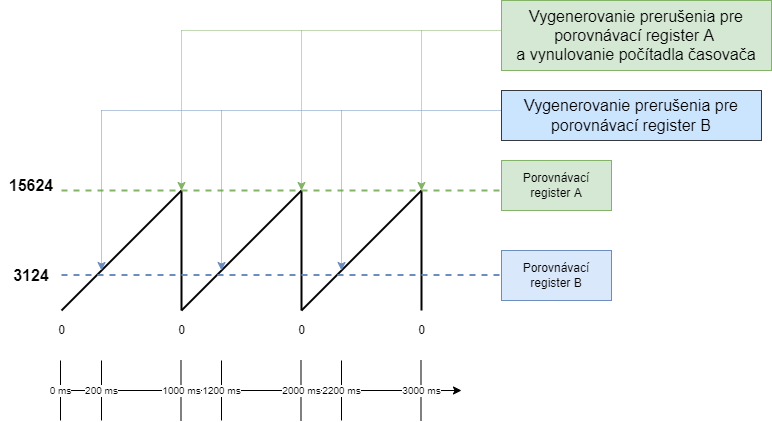
\includegraphics[width=0.85\textwidth]{img/ctc-timer-value.png}
    \caption{Zmena hodnoty časovača v CTC móde}
    \label{figure:ctc-timer-value}
\end{figure}

Pseudokód daného riešenia vyzerá nasledovne:

\begin{lstlisting}[
    label={lst:ctc-interrupt},
    language=c]  

Enable timer Compare nad Capture A interrupt
Enable timer Compare nad Capture B interrupt
Enable global interrupts

Set Output Compare Register A value to 15624
Set Output Compare Register B value to 3124

Set timer mode to CTC
Set timer prescaler to 64

WHILE forever
END WHILE

ISR Compare nad Capture A
    // Do some work at 1 second interval
END ISR

ISR Compare nad Capture B
    // Do some work at 200 milliseconds interval 
END ISR

\end{lstlisting}

Poznamenať by sme mali, že pri použití CTC módu nie je možné nastaviť časovač tak, aby generoval akékoľvek dva, resp. tri intervaly. Pre časovač je možné nastaviť
len jednu preddeličku. Z toho vyplýva, že aj všetky intervaly musia byť kompatibilné s danou preddeličkou. Ak náš predchádzajúcu príklad trochu upravíme
a 200 milisekundový interval nahradíme 250 milisekundovým dostaneme spomínané nekompatibilné hodnoty. Pomocou vzorca \ref{eq:register-value} sa pokúsime vypočítať
porovnávaciu hodnotu:
\begin{equation}
    \begin{aligned}
        Hodnota\:registra & = (\frac{Frekvencia\:hodín}{Preddelička \times Cieľová\:frekvencia}) - 1 \\
                          & = (\frac{1 \times 10^{6}}{64 \times 4}) - 1                              \\
                          & = (\frac{1 \times 10^{6}}{256}) - 1                                      \\
                          & = 3906,25 - 1                                                            \\
                          & = 3905,25                                                                \\
    \end{aligned}
\end{equation}

Vidíme, že výsledkom nie je celé číslo. Teoretickým riešením by mohlo byť zaokrúhlenie danej hodnoty na celé číslo. Tým by sme však do celého procesu vniesli nepresnosť,
ktorá je vo väčšine prípadov neakceptovateľná.

\subsubsection{PWM mód}
\noindent \par
Pulse Width Modulation (impulzová šírková modulácia) alebo aj PWM je technika, pomocou ktorej je možné ovládať analógové zariadenia pomocou digitálneho signálu.
Jednoduchým príkladom je stmievanie led žiarovky alebo ovládanie rýchlosti motora. PWM signál nie je reálnym analógovým signálom, len ho určitým spôsobom dokáže napodobniť.
Pomocou digitálneho ovládania dokážeme rýchlo napájanie vypínať alebo zapínať a riadiť tak prúd dodávaný do zoriadenia. Ak necháme prúd zapnutý dlhší čas ako čas, v ktorom
je vypnutý, tak zvýšime priemernú úroveň výkonu. V opačnom prípade priemernú úroveň výkonu znížime. Trvanie „času zapnutia“ sa nazýva šírka impulzu.
Ak chceme získať rôzne analógové hodnoty, zmeníme šírku impulzu. Na vyjadrenie dĺžky času zapnutia sa používa termín Duty cycle (pracovný cyklus). Udáva sa v percentách
a hovorí o dĺžke „času zapnutia“  počas jedného intervalu \cite{WhatPWMSignal}.
\begin{figure}[!h]
    \centering
    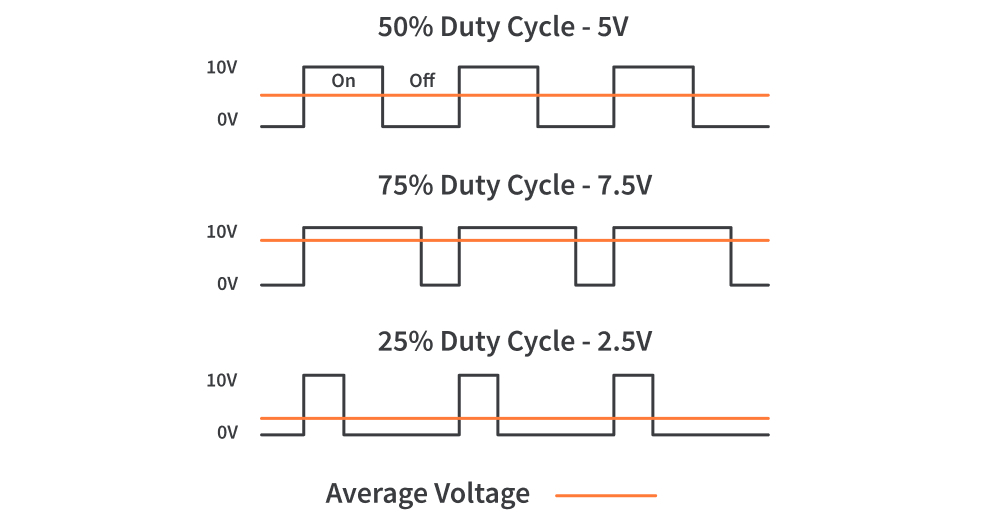
\includegraphics[width=0.85\textwidth]{img/duty-cycle.jpg}
    \caption{Ukážka rôznej hodnoty striedy v PWM signále}
    \source{\cite{WhatPWMSignal}}
    \label{figure:pwm-signal}
\end{figure}

Ako sme si ukázali, pre generovanie PWM signálu potrebujeme neustále v určitých časových intervalov „vypínať“ a „zapínať“ prúd. Na to môžu výborne poslúžiť časovače.
Tie dokážu na presne dané piny mikrokontroléra zapisovať logickú jednotku, resp. nulu čoho výsledkom môže byť PWM signál. To je možné docieliť
pomocou špeciálnych PWM módov, ktoré si predstavíme v ďalšej časti diplomovej práce.

\noindent \par
Fast PWM mód je jedným z podporovaných modov v AVR časovačoch. V tomto móde sa časovač jednoducho počíta od 0 po maximálnu kapacitu registra. Pri počítaní porovnáva svoju hodnotu, s hodnotami v porovnávacích registroch.
Používajú sa rovnaké porovnávacie registre ako v už spomínanom CTC móde. Tieto registre sú naviac namapované na externé piny mikrokontroléra.
Na výstupné piny je zapísaná logická jednotka, keď je časovač na 0 a logická nula, keď sa časovač zhoduje s výstupným porovnávacím registrom. Čím vyššia je hodnota
v porovnávacom registri, tým je na pine nastavená väčšia strieda \cite{shirriffSecretsArduinoPWM}. \par
Existujú aj rôzne variácie Fast PWM módu, kedy je možné nastaviť maximálnu hodnotu časovača a tým meniť frekvenciu. \par
Na obrázku č.\ref{figure:fast-pwm-mode} môžeme vidieť zmenu hodnoty v 8 bitovom AVR časovači spolu s PWM signálom, ktorý je schopný vygenerovať.
\begin{figure}[!h]
    \centering
    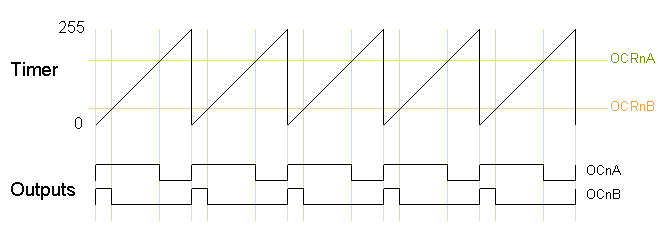
\includegraphics[width=0.85\textwidth]{img/fast-pwm-graph.png}
    \caption{Fast PWM mód použitý v 8 bitovom časovači}
    \source{\cite{shirriffSecretsArduinoPWM}}
    \label{figure:fast-pwm-mode}
\end{figure}

Porovnávací register A je vyznačený zelenou farbou, zatiaľ čo register B je označený farbou červenou. Obrázok č.\ref{figure:fast-pwm-mode} znázorňuje následné hodnoty:
\begin{itemize}
    \item Porovnávací register A
          \subitem{Hodnota porovnávacieho registra A: 180}
          \subitem{Strieda pre porovnávací register A: (180 + 1)/256 = 70,7\%}
    \item Porovnávací register B
          \subitem{Hodnota porovnávacieho registra B: 50}
          \subitem{Strieda pre porovnávací register B: (50 + 1)/256 = 19,9\%}
\end{itemize}

Pri výpočte striedy si možeme všimnúť, že k hodnote v registri sme pripočítali 1. Je to kvôli tomu, že AVR časovaču trvá jednu periódu navyše pokiaľ hodnotu
na danom pine zmení \cite{shirriffSecretsArduinoPWM}.

\noindent \par
Ďalším módom je tzv. Phase-Correct PWM mód. V tomto móde časovač počíta od 0 po maximálnu hodnotu registra a následne sa hodnota nevynuluje
ale časovač znovu počíta od najväčšej hodnoty po 0. Na výstupné piny je zapísaná logická jednotka, keď je časovač na 0. Pri počítaní smerom nahor sa pri dosiahnutí porovnávacieho registra výstupný pin vypne
a následne pri počítaní smerom nadol zapne. Výsledkom je symetrický výstup \cite{shirriffSecretsArduinoPWM}. Na obrázku  č.\ref{figure:phase-correct-pwm-mode} si môžeme všimnúť,
že dôsledkom počítania aj smerom nadol je polovičná frekvencia oproti režimu Fast PWM.

\begin{figure}[!h]
    \centering
    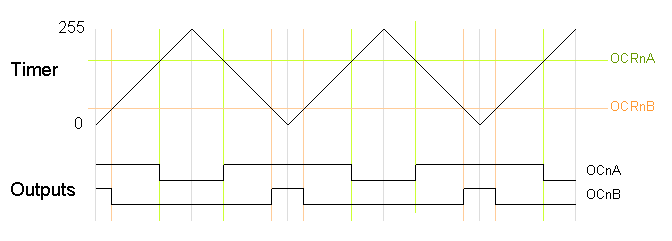
\includegraphics[width=0.85\textwidth]{img/phase-correct.png}
    \caption{Phase-Correct PWM mód použitý v 8 bitovom časovači}
    \source{\cite{shirriffSecretsArduinoPWM}}
    \label{figure:phase-correct-pwm-mode}
\end{figure}

Porovnávací register A je vyznačený zelenou farbou, zatiaľ čo register B je označený farbou červenou. Obrázok č.\ref{figure:phase-correct-pwm-mode} znázorňuje následné hodnoty:
\begin{itemize}
    \item Porovnávací register A
          \subitem{Hodnota porovnávacieho registra A: 180}
          \subitem{Strieda pinu porovnávaceho registra A: (180 + 1)/256 = 70,7\%}
    \item Porovnávací register B
          \subitem{Hodnota porovnávacieho registra B: 50}
          \subitem{Strieda pinu porovnávaceho registra B: (50 + 1)/256 = 19,9\%}
\end{itemize}
